% vim: tw=99

\documentclass{article}

\usepackage{fancyhdr}
\usepackage{hyperref}
\usepackage{listings}
\usepackage{minted}
\usepackage[style=numeric-comp]{biblatex}
\usepackage{booktabs}
\usepackage{graphicx}

\addbibresource{references.bib}

\graphicspath{{images/}}

\providecommand*{\listingautorefname}{Listing}
\renewcommand{\sectionautorefname}{Section}

\pagestyle{fancy}
\lhead{\leftmark}
\chead{}
\rhead{}

\begin{document}

\title{ScPy: A SuperCollider Extension for Performing Numerical Computation via Embedded Python}

\author{Noah Weninger \and Abram Hindle}

\maketitle

\begin{abstract}

    SuperCollider~\cite{wilson2011supercollider}, a language for sound synthesis and algorithmic
    composition of audio, supports a wide range of synthesis, effect and analysis algorithms.
    However, available operations are limited to those implemented explicitly as Unit Generators
    (UGens). Since UGens are written in C/C++ and loaded as plugins during the SuperCollider server
    boot process, it is impossible to live code UGens, which limits the user to creating sound as a
    composition of existing UGens during a performance.  Many of the vector operations required for
    efficiently creating complex audio effects are notably missing or tedious to use. To overcome
    this, we present ScPy, a UGen which embeds Python within SuperCollider to enable the use of the
    optimized vector operations provided by the NumPy library.

\end{abstract}

\section{Introduction}\label{sec:introduction}

Although a number of open-source projects which interface other languages with SuperCollider exist
\cite{systemsinterfacingwithsc,magnusson2011ixi,orlarey2009faust}, they are mostly SuperCollider
clients, which have features to control synths and send other automation messages.  One notable
exception is OctaveSC~\cite{octavesc}, which embeds GNU Octave within SuperCollider.  However, it
is designed for performing operations on control rate data arrays and suffers from performance
issues which prevent it from being used on audio rate data.

One of the goals of this project is to enable more flexible experimentation with FFT and phase
vocoder based operations. SuperCollider contains a total of 32 built in phase vocoder operations,
which provide the ability to produce many simple effects. There are additionally some extra
operations available as user created extensions. However, many conceivable effects are impossible,
including basic phase vocoder effects such as pitch shifting. Some examples of novel effects can
be found in~\autoref{sec:usage}.

ScPy enables users to overcome these limitations. By embedding the Python programming language
within SuperCollider, it is possible to do numerical processing operations which would be too slow
to perform in real time with SuperCollider alone. Through access to the NumPy library, previously
difficult or impossible phase vocoder operations become trivial. Although our usage of this library
for testing purposes has mostly focused on FFT based operations, support exists for passing
arbitrary data buffers to Python, which can be used to process numerical data for many other
purposes as well.

ScPy is developed and maintained as an open-source project under the GPLv3 license. The latest code
and documentation is available on GitHub\footnote{\url{https://github.com/nwoeanhinnogaehr/ScPy}}.

\section{Methodology}\label{sec:methodology}

During the initial planning stage of the project, we wanted to essentially provide a set of
fundamental operations on spectral data which could be composed together to perform any conceivable
effect. It was also a requirement that these operations would be syntactically concise to enable
easy and fast experimentation. Ideally, the system would be able to handle complex effects in
real-time.

ScPy is unlike many New Instruments for Musical Expression (NIMEs) because it does not have the
properties of any traditional instrument. However, it can still be considered a NIME because it
ultimately is a tool to enhance musical expression, just with an unconventional method of
interaction.  Dimension space analysis, as explored by Birnbaum et al.~\cite{birnbaum2005towards},
can facilitate the comparison of use cases for NIMEs.

\begin{figure}[h]
\caption{NIME dimension space analysis for ScPy.}
\vspace{1em}
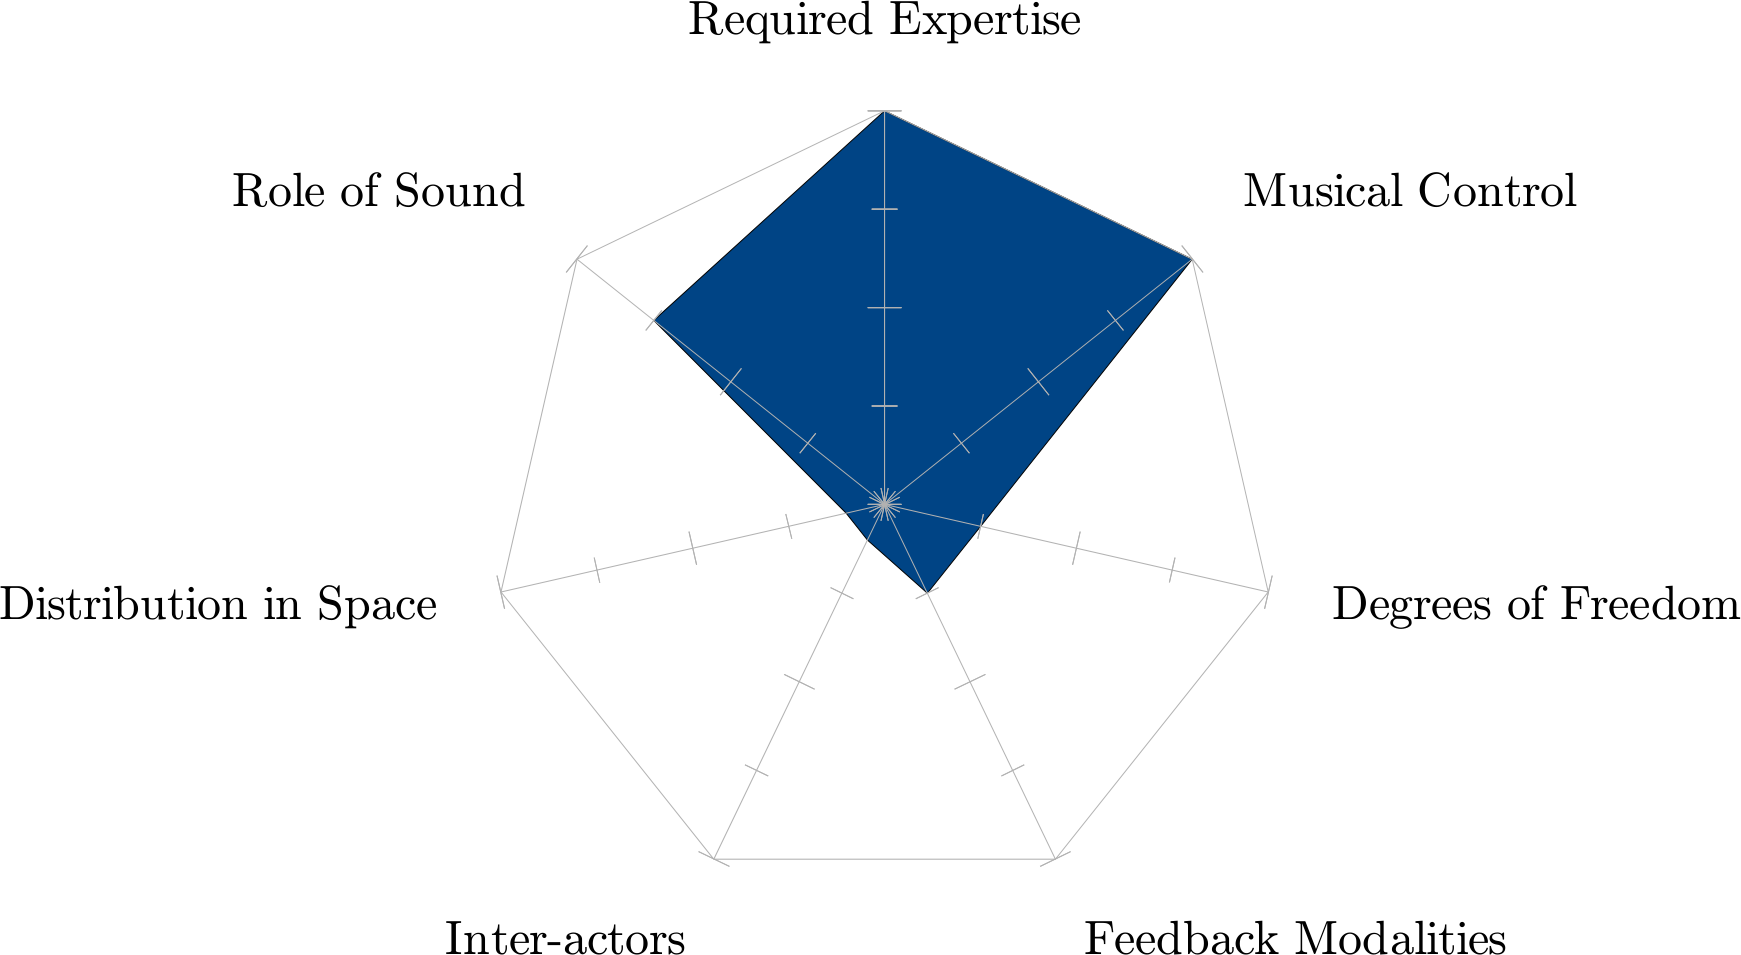
\includegraphics[scale=0.2]{nime-plot}
\label{fig:nime}
\end{figure}

Although designing a domain-specific language (DSL)~\cite{van2000domain} for this task was briefly
considered, we eventually decided to use Python for a number of reasons. First, Python includes an
excellent C API which makes embedding it within other languages trivial in comparison to many other
options.  Second, Python's syntax is easily readable and concise --- it clearly adheres to our
goals. Finally, Python has a massive number of community built libraries for performant scientific
and numerical computing. With a few small exceptions, which are clearly specific to spectral data
(such as the phase vocoder), these libraries contained every one of the fundamental operations we
could think of.

It may seem as though embedding an interpreted language within an interpreted language could offer
no performance advantage. There is certainly some performance hit when switching languages and
transferring data. However, the biggest advantage comes not strictly from performance but from the
diversity of operations which become available with highly optimized implementations. NumPy is used
internally by ScPy for handling data arrays, so the entire NumPy library of mathematical functions
comes at no cost.  Any other Python library can easily be imported as well. Limited experiments
have been done with the SciPy library. It would also be possible to use Theano to do processing on
the GPU for extra performance. Implementing an equivalent to these popular Python libraries in pure
SuperCollider is certainly possible, but it would require a very large amount of work and would see
no adoption outside of the audio computing community.

\section{Usage}\label{sec:usage}

Use of ScPy is through the classes \texttt{Py} and \texttt{PyOnce}. \texttt{Py} is used for
processing real-time data, and \texttt{PyOnce} is used for doing initialization or other one time
processing. Both have one required argument, a block of Python code. A map of variable names may
optionally be provided to bind SuperCollider variables to Python variables.  Additionally, there is
an optional \texttt{DoneAction} argument which specifies an action to occur in SuperCollider after
the Python code has finished executing.

\begin{listing}[H]
    \begin{minted}[linenos=true]{SuperCollider}
(PyOnce("
    # comments in Python have different syntax!
    print('Hello from Python!')
    print('x is', x)
", (x: 62)))
    \end{minted}
    \caption{Hello world with ScPy.}
    \label{lst:helloworld}
\end{listing}

\begin{listing}[H]
    \inputminted[linenos=true]{SuperCollider}{../examples/template.sc}
    \caption{SuperCollider boilerplate for no-op FFT effect with ScPy.}
    \label{lst:boilerplate}
\end{listing}

When \autoref{lst:boilerplate} is run, an anonymous synth is created which will take in audio
from an external source, perform an STFT, process the spectral data with ScPy, perform an inverse
STFT, then finally output the resulting audio. Lines 8--9 contain Python code defining the
processing function where operations are to be inserted. Further examples will replace only those
lines. Line 16 contains the Python code to convert the spectrum into a NumPy array, process it,
then write back the processed version.

A special function, \texttt{out}, is provided to mutate data in SuperCollider buffers. It takes a
variable which is bound to a \texttt{Buffer} or \texttt{FFT} object and a new value. The buffer is
modified in place to hold the new data.

\begin{listing}[H]
    \begin{minted}[linenos=true]{python}
pv = PhaseVocoder(hop)

def fn(x):
    x = pv.forward(x)
    idx = indices(x.shape)[1]
    x = pv.shift(x, lambda freq:
        freq * (0.8 + mod(-time + 0.1*idx, 10)*0.045))
    x = pv.backward(x)
    return x
    \end{minted}
    \caption{A novel effect to transform any sound into a falling Shepard tone. This example makes
    use of the phase vocoder \texttt{shift} operation, which applies a function to frequency, then
    reorganizes the spectrum to move the new frequencies into the appropriate bins.}
    \label{lst:shepard}
\end{listing}

\begin{listing}[H]
    \begin{minted}[linenos=true]{python}
pv = PhaseVocoder(hop)

def fn(x):
    x = pv.forward(x)
    x = pv.to_bin_offset(x)
    x.imag = -x.imag
    x = pv.from_bin_offset(x)
    x = pv.backward(x)
    return x
    \end{minted}
    \caption{An effect which inverts the frequency of each analysis bin across the center of
    the bin, creating an unusual detuning effect.}
    \label{lst:binflipper}
\end{listing}

\section{Implementation}\label{sec:implementation}

ScPy is written mostly in C++, but with a small SuperCollider class library to connect the C++
back-end, and a small Python library that provides some useful operations. Due to differences
between these languages, connecting them was somewhat awkward in some cases.

Since UGens may only be used as part of a synth, \texttt{PyOnce} is provided as a wrapper which
hides this detail from the user and allows the execution of Python code outside of a synth. It is
useful for doing initialization work. Since the current implementation executes Python code in a
single global namespace, a typical usage patten is for state to be defined in a \texttt{PyOnce}
block which is later accessed and modified in a \texttt{Py} block.

One issue involves the process of passing data between SuperCollider and C++. Since UGens are
designed to work primarily with data streams, adding support for passing in many types of data came
with a number of challenges. Essentially, all data must be serialized into an array of floats.
Strings must be converted to an array of ASCII character codes, and prepended with their length.
Arguments passed through to the Python code can have one of many types, and therefore type
information must be encoded as well. However, just passing the type of a variable is not enough to
know what we can do with it, since we also want to know if it inherits from a class we can use.

Since \texttt{FFT} objects in SuperCollider operate on a single channel only, they must be placed
in \texttt{Array} objects to support multichannel audio. \texttt{Array}s can hold objects of any
type, so it is natural to convert them to Python \texttt{list} objects, which have similar
properties. However, this presents an interesting problem: multichannel \texttt{FFT} objects are
then converted to \texttt{list}s of \texttt{ndarray} objects in Python. These are a bit more
awkward to work with than basic \texttt{ndarray} objects, but can easily be converted using a call
to the \texttt{array} function in Python. This can be seen in practice on line 16 of
\autoref{lst:boilerplate}. Although it would be possible to do this conversion
automatically, it is left out for the purpose of not introducing a feature simply to work around an
incomplete implementation of \texttt{FFT} objects in SuperCollider. The current conversions will
continue to function as intended if \texttt{FFT} objects are given multichannel support in the
future.

\begin{table}[H]
    \caption{Type correspondence between SuperCollider and Python}
    \begin{center}
        \begin{tabular}{ll}
            \toprule
            SuperCollider type & Python type \\
            \midrule
            \texttt{Float} & \texttt{float} \\
            (subclass of) \texttt{UGen} & \texttt{ndarray} of \texttt{float} \\
            \texttt{Buffer} & \texttt{ndarray} of \texttt{float} \\
            \texttt{FFT} & \texttt{ndarray} of \texttt{complex} \\
            \texttt{Array} & \texttt{list} \\
            \bottomrule
        \end{tabular}
    \end{center}
\end{table}

As shown in \autoref{lst:shepard} and \autoref{lst:binflipper}, ScPy includes a phase vocoder
implemented in Python for performing frequency transformations. Interestingly, although all of
SuperCollider's FFT operations are referred to as phase vocoder operations, there is actually no
implementation of a phase vocoder to be found in the SuperCollider code base at the time of
writing. It is likely that a phase vocoder was once intended to be implemented, but the 32
so-called phase vocoder effects are simply transformations to the Cartesian or polar
representations of the spectrum.

\section{Future Work}

At the time of writing, ScPy only supports handling audio rate data via SuperCollider's
\texttt{Buffer} objects. In order to make some use cases more ergonomic, ScPy could certainly be
extended to support raw audio rate input. For example, this would make time domain audio data even
simpler to work with than frequency domain data is currently. It would also enable SuperCollider's
FFT UGen to be easily re-implemented in Python for greater flexibility.

Support for more SuperCollider types, such as events or strings, could be added to open up ScPy to
more use cases.

Multi-core processing support would allow for many more sounds to be processed in real-time.

Creating a more generic extension which supports many languages would have a number of advantages.
One option for implementing this would be to define a specification to communicate and share data
with a generic UGen in a running SuperCollider instance.

Although extending SuperCollider was the focus of this project, similar improvements could be made
to the CSound\cite{boulanger2000csound,lazzarini2005extensions}, Chuck\cite{wang2008chuck} or
Faust\cite{orlarey2009faust} environments as well.

\printbibliography{}

\end{document}
